\chapter{General Introduction}

\epigraph{\textit{Natural selection cannot possibly produce any modification in any one species exclusively for the good of another species.}}{--- \textup{Charles Robert Darwin}}

\minitoc[n] % minitoc without title

% We will volontarily be vague at time. Please bear with us

\section{The Evolution of Cooperation}

  \subsection{The Problem of Evolving Cooperation}

    Among social behaviours, cooperation is one that appears to be the most prevalent in nature. Its examples and practical occurences are as diverse as central in numerous species. Furthermore, it is also argued that cooperation is one of the leading factors in most of the major transitions in evolution (e.g. the appearance of eukaryotes or the evolution of multicellularity)~\parencite{Szathmary1995}. The classical definition of cooperation in evolutionary biology is as follows: cooperation is a behaviour where an \emph{actor} (the individual who initiates the behaviour) behaves in such a way that is beneficial to a \emph{recipient}~\parencite{West2007a}. Given how broad this definition is, numerous biological phenomena can be included under this label. 

    Cooperation is present at every level of the natural world. Even unicellular organisms such as bacteria and microorganisms are known to frequently act in a cooperative manner. By using secretions, microorganisms are capable of collective sharing and communication~\parencite{Elena2003, Keller2006, West2006}. \emph{Pseudomonas aeruginosas} for example produce nutrients that every organism in the vicinity can benefit from~\parencite{Popat2012, Harrison2013}. Insects from the Hymenoptera (e.g. ants, wasps, bees) and Isoptera (e.g. termites) are known for the presence of \emph{eusociality} (Figure~\ref{fig:CooperationExamples}~(A))~\parencite{Wilson1990} which entails highly cooperative behaviours between individuals. In particular, the most distinctive feature of eusociality is the existence of division of reproductive labor. This means that reproductive and non-reproductive castes (e.g. worker caste) coexist, where individuals which cannot reproduce care for the youngs of others. Some social carnivores are capable of collective hunting, where several members of the same group coordinate their actions to catch a challenging prey. Spotted hyenas (see Figure~\ref{fig:CooperationExamples}~(B)) in particular are efficient hunters who rely on signaling and communication to coordinate~\parencite{Drea2009a, Smith2010, Smith2012a} and are able to defend their catch against lions. But they are also considered to be the most social taxon among Carnivora~\parencite{Mills2003} and the complexity of their social organization is comparable to that of primates~\parencite{Drea2003}. Finally, the scope of cooperative behaviours is such that even cooperation between individuals from different species (i.e. interspecific cooperation) is abundant~\parencite{Bshary2004}. Cleaning symbiosis, where a "client" has its teeth or body cleaned from parasites or dead tissues by a smaller "cleaner"~\parencite{Poulin1996}, is an example of this form of cooperation. In particular some fishes, especially \emph{Labroides dimidiatus} (wrasses, Figure~\ref{fig:CooperationExamples}~(D)), are known to clean other bigger fishes to the point that there exists "cleaning station" where multiple aquatic animals converge to enjoy their services.


    % Much higher on the size scale is a popular textbook example of social behaviours: ants~(Figure~\ref{fig:CooperationExamples}~(A)). More generally, the presence of \emph{eusociality} in the animal world is an astonishing display of cooperative features~\parencite{Wilson1990}. While ants are among the most well-known examples, insects from the Hymenoptera (i.e. ants, wasps, bees) and Isoptera (i.e. termites) orders are all eusocial and represent most of the insect biomass\parencite{Wilson2008}. It is interesting to note that two rodent species, the naked mole-rat and the Damaraland mole-rat, are the only vertebrates to have achieved eusociality. Eusociality might be defined as one of the highest levels of sociality and displays several impressive examples of highly advanced cooperative actions. For example, there is cooperative care of youngs in eusocial societies, which means that individuals help raise offspring which are not their own. Also, eusocial insects are capable of achieving efficient division of labour, a cooperative trait where individuals specialize between several roles, either to achieve several tasks simultaneously or to coordinate more efficiently. In particular, division of labour is often permanent and comes with strong morphological differences between specialized individuals. Last but not least, eusociality is also defined by the division of reproductive labor. This means that there exists reproductive and non-reproductive castes (e.g. the worker caste), which is an extreme form of cooperation between these individuals. Because of all of these reasons, an ants colony is often viewed as a particular superorganisms wherein individuals work as one for the benefit of the group.

    % However, this also means that some organisms could profit from these nutrients without having to produce anything themselves (given that production is costly). This is where a problem of public goods can arise: because "cheaters"\footnote{The term "cheaters" will appear several times along the lines of this manuscript. Because this word has a particular bad connotation with regards to human actions, it may be misunderstood that we attribute a malevolent intention to the organisms. Rather, through the rest of the manuscript, It should be understood as "one that profits from a benefit without paying any cost".} can benefit from these nutrients without contributing themselves. Interestingly, these situations are well studied in the realm of cooperative dilemma, as in economics for example.
    
    
    % , which proves how complex these cooperative interactions in microorganisms are. It would also not be so far-stretched to consider that the complex network of genes interactions, where genes act together to build complex living machines may very well fall under the umbrella of cooperation. It is even more astonishing when we consider that those genes used to be independent replicators living freely~\parencite{Dawkins1976, Szathmary1995}. Finally, and in a similar fashion as our previous example, multicellularity is a perfect display of high cooperation between numerous different organisms. The birth of multicellular organisms is explained by the fact that single prokaryotic organisms gathered and where incorporated as mitochondries in what are now eukaryotic cells to form complex multicellular organisms. Szathmary \& Maynard Smith considered this cooperative transition to multicellularity as one of the major transitions in evolution~\parencite{Szathmary1995}.

    \begin{figure}[hbt]
        \begin{center}
          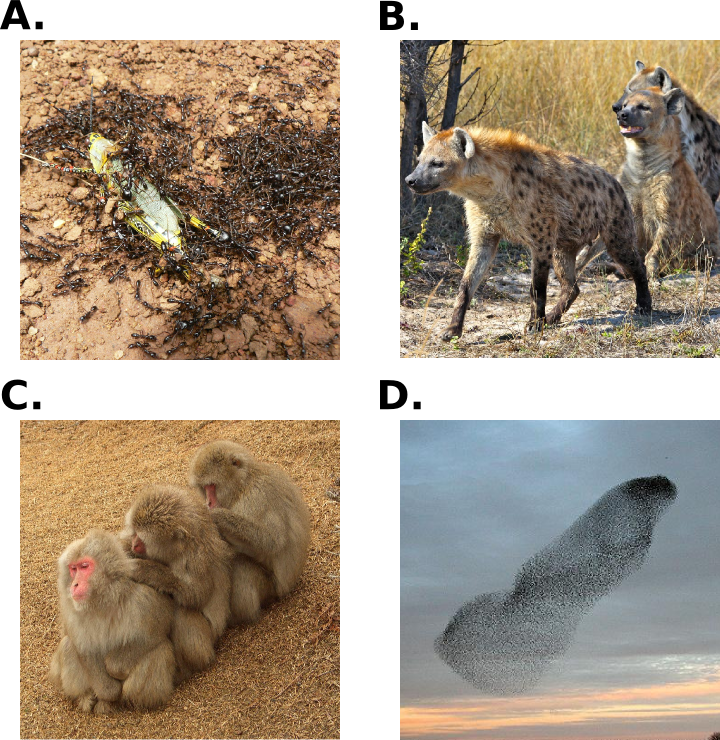
\includegraphics[scale = 0.5]{fig/Intro/CooperationExamples.png}
          \caption{\textbf{Multiple aspects of cooperation.} {\em (A)}~Eusocial insects like Hymenoptera (e.g. ants) are capable of highly developed cooperative behaviours. {\em (B)}~Some social carnivores like the spotted hyena perform various cooperative behaviours and are capable of advanced coordination strategies during collective hunts. {\em (C)}~Social grooming is a cooperative behaviour where individuals will groom each other reciprocally (here shown in impalas). {\em (D)}~Interspecific cooperation (or mutualism) is common among cooperative behaviours. Here we show a \emph{Labroides dimidiatus} involved in a cleaning symbiosis where the individual cleans another from parasites.}
          \label{fig:CooperationExamples}
        \end{center}
    \end{figure}

    % Much higher on the size scale is a popular textbook example of social behaviours: ants~(Figure~\ref{fig:CooperationExamples}~(A)). More generally, the presence of \emph{eusociality} in the animal world is an astonishing display of cooperative features~\parencite{Wilson1990}. While ants are among the most well-known examples, insects from the Hymenoptera (i.e. ants, wasps, bees) and Isoptera (i.e. termites) orders are all eusocial and represent most of the insect biomass\parencite{Wilson2008}. It is interesting to note that two rodent species, the naked mole-rat and the Damaraland mole-rat, are the only vertebrates to have achieved eusociality. Eusociality might be defined as one of the highest levels of sociality and displays several impressive examples of highly advanced cooperative actions. For example, there is cooperative care of youngs in eusocial societies, which means that individuals help raise offspring which are not their own. Also, eusocial insects are capable of achieving efficient division of labour, a cooperative trait where individuals specialize between several roles, either to achieve several tasks simultaneously or to coordinate more efficiently. In particular, division of labour is often permanent and comes with strong morphological differences between specialized individuals. Last but not least, eusociality is also defined by the division of reproductive labor. This means that there exists reproductive and non-reproductive castes (e.g. the worker caste), which is an extreme form of cooperation between these individuals. Because of all of these reasons, an ants colony is often viewed as a particular superorganisms wherein individuals work as one for the benefit of the group.

    % If we unzoom again the lens with which we look at the world, we can find other powerful examples of cooperation among bigger vertebrates. Numerous species have evolved strong sociality, or presociality, which gives the opportunity to watch impressive cooperative actions in the animal world. For example, social carnivores are capable of collective hunting, where several members of the same group will coordinate their actions to catch a particularly difficult or quick prey. For examples, lions are famously known for their communal and highly cooperative behaviours of collective hunting, for which they are capable of division of labour~\parencite{Scheel1991, Stander1992}. Less well-known but as much impressive, spotted hyenas~(Figure~\ref{fig:CooperationExamples}~(B)) also demonstrate high level of coordination in their collective hunting habits. While often wrongly considered but a scavenger, hyenas are also great hunters who rely on signaling and communication to coordinate~\parencite{Drea2009a, Smith2010, Smith2012a} and are capable of defending their catch against lions. The behaviours of those predators could easily be considered as complex tactics by a human observer. But even without being concerned with something as brutal as hunting, social carnivores tend to live, as their name suggests, in highly cooperative societies. To go on with the example of spotted hyenas, they are in particular considered to be the most social among Carnivora~\parencite{Mills2003} and the complexity of their social organization is comparable to that of primates~\parencite{Drea2003}. They live in a matriarchal societies where the females dominate the males and enforce the hierarchy through agression. Non-dominant females also take care of the youngs of other females higher in the hierarchy, something which is known as alloparenting and can also be found in primates~\parencite{Small1990} and in other carnivores~\parencite{Packer2001}. Among several social species, individuals also engage in social grooming~(Figure~\ref{fig:CooperationExamples}~(C)), where they will clean each other and which is an important bounding activity which strengthen the social structure of the group~\parencite{Spruijt1992}. Finally, we can also quickly mention the behaviours of sentinels, for example in birds like the Arabian babbler~\parencite{Wright2001} or meerkats~\parencite{CluttonBrock1999}. Individuals who adopt these behaviours will act as watchers for other individuals in their group, responsible for looking for predators approaching and warn the other individuals, sometimes thus taking the risk of attracting attention to themselves.

    % It is also easy to be amazed by the collective motion of flocks of birds~(Figure~\ref{fig:CooperationExamples}~(D)). Animals might sometimes organize into flocks, herds or schools from which will emerge a collective behaviour~\parencite{Couzin2002, Couzin2003}. In particular, what is impressive is that the collective cohesion achieved is due to individual behaviours which do not depend on high cognitive abilities and does not require a particular central decision. These social behaviours are beneficial to the individuals that constitute the groups because it can for example increase group vigilance, confuse predators, decrease the risk for each individual to be attacked or even allow to organize an active defense against a predator~\parencite{Hamilton1971, Olson2013}.

    % For the moment we simply gave examples of cooperation between members of the same species (intraspecific cooperation). Yet if we again look at a higher scale we can also observe numerous displays of cooperation between individuals of different species (interspecific cooperation). Often called mutualism (as we explain later), this form of cooperation is abundant~\parencite{Bshary2004}. For example, most plants require pollinators in order to transport their pollen so that they can succesfully pollinate the flowers. In exchange, the pollinators, whose most representative are insects, gain nectar as a benefit. Another example is that of cleaning symbiosis, where a "client" has its teeth or body cleaned from parasites or dead tissues by another smaller "cleaner"~\parencite{Poulin1996}. For example, some fishes, especially wrasses, are known to often clean other bigger fishes, to the point that there exists "cleaning station" where multiple aquatic animals converge to enjoy their services. The yellow-billed oxpecker also regularly eats insects and ticks from the back of mammals. The gut flora of some animals, human beings among them~\parencite{Backhed2005}, is also another example of strong interspecific cooperation, as it is constituted of up to 100 trillion of microorganisms that help process food.

    % % KILLER WHALES ? Domestication ?

    % % On peut en dire plus sur les humains mais j'ai pas les références pour le moment.

    % In conclusion, in nearly every different levels of complexity in the living world, we can find examples of cooperative actions. More importantly, cooperation is not only present but also appears to be one of the leading factors in every major transitions in evolution~\parencite{Szathmary1995}. Moreoever, we did not touch upon human cooperation until now but it is obvious that human beings are very strong cooperators. In particular, cooperation is at the basis of the construction of our social structure and social sciences have been for long interested in studying human cooperation~\parencite{West2011a}. Therefore there is particular interest in trying to explain how could cooperation evolve and give rise to so much diversity in social behaviours today. 

    Yet explaining the evolution of cooperation has been one of the major challenges in evolutionary biology~\parencite{Hamilton1964, Dugatkin2002, West2011a}. Charles Darwin, as shown by the epigraph of this chapter, had already argued that the evolution of cooperation could pose a problem to his theory. He thought that the existence of a non-reproductive caste in eusocial insects was "one special difficulty, which at first appeared to me to be insuperable, and actually fatal to my whole theory"~\parencite{Darwin1859}. According to the theory of evolution, life is a struggle where only the \emph{fittest individuals} survive. The main purpose of evolutionary biology is to explain adaptation~\parencite{West2011a}. In particular, natural selection is driven by the reproduction of individuals. Namely, because transmission of genetic material occurs through reproduction, evolution leads to an increase in genes and traits that increase the relative number of offspring (i.e. fitness) of the organism. This is where this understanding of adaptation appears to contradict the evolution of cooperation.

    % For example, a individual that acts as a sentinel for the group takes the risk of being spotted more easily by a predator, thus paying a hefty cost for the good of the others.

    % However, this also means that some organisms could profit from these nutrients without having to produce anything themselves (given that production is costly). This is where a problem of public goods can arise: because "cheaters"\footnote{The term "cheaters" will appear several times along the lines of this manuscript. Because this word has a particular bad connotation with regards to human actions, it may be misunderstood that we attribute a malevolent intention to the organisms. Rather, through the rest of the manuscript, It should be understood as "one that profits from a benefit without paying any cost".} can benefit from these nutrients without contributing themselves. Interestingly, these situations are well studied in the realm of cooperative dilemma, as in economics for example.


    But cooperation is defined as a behaviour that benefits another individual than the actor. One must keep in mind that "costs" and "benefits" refer to the fitness of the individual (i.e. the number of this individual's offspring) and not direct material elements. In consequence, it decreases the relative fitness of the actor compared to that of others in the population and should then be selected against. In particular, cooperative individuals are under the threat of invasion from cheaters (or freeloaders\footnote{The terms "cheaters" and "freeloaders" will appear several times along the lines of this manuscript. Because this word has a bad connotation with regards to human actions, it may be misunderstood that we attribute a malevolent intention to the organisms. Rather, through the rest of the manuscript, tt should be understood as "one that profits from a collective benefit without paying any cost".}). To illustrate this issue, let us take back the example of \emph{P. aeruginosas} which we previously talked about. Let's imagine a population constituted of cooperators which can pay a certain cost to give a benefit to others. A given individual can benefit from every individuals in the population and the situation appears ideal. However, say now that a mutant, which does not cooperate, appears in the population. Then this mutant can benefit from the cooperative actions of others without having to pay any cost. From this it stems that its relative fitness will be higher than that of cooperators. In consequence, it will produce more offspring and mutants will begin to invade the population. The process will repeat itself as cheaters always have a higher fitness than cooperators until no cooperators are left in the population. From this comes that cooperation should not be able to exist. 

    Biologists have therefore been studying the mechanisms which could explain the evolution of cooperation for several decades. Because cooperative actions are so diverse, numerous models have been proposed to classify the different mechanisms which could explain the adaptation of cooperative traits~\parencite{Dugatkin2002, Keller2006, Bergmuller2007a, West2007}. For our overview of cooperation in this present manuscript, we follow the classification of West and colleagues~\parencite{West2007a}. In particular, these mechanisms can be classified in two main categories: \emph{direct fitness benefits} and \emph{indirect fitness benefits}.

     % (see Figure~\ref{fig:ClassificationCooperation}).

    % \begin{figure}[hbt]
    %     \begin{center}
    %       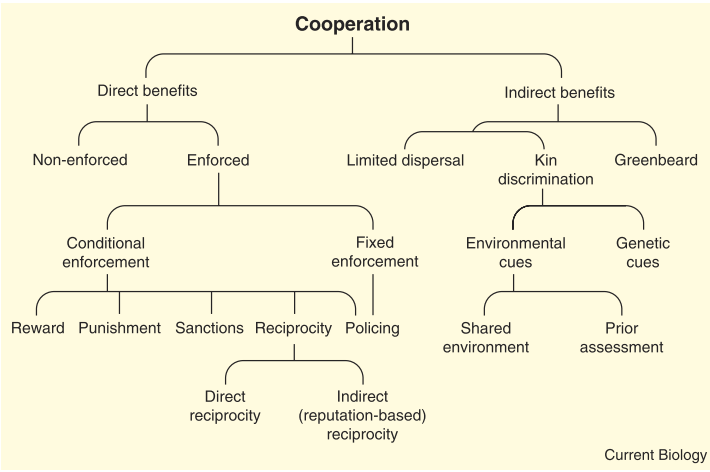
\includegraphics[scale = 0.50]{fig/Intro/ClassificationCooperation.png}
    %       \caption{\textbf{Classification of the mechanisms behind the evolution of cooperation.} Numerous classifications for the explanation of the evolution of cooperative actions have been proposed. However, most people agree that those explanatations can be divided into two categories: direct benefits and indirect benefits. Inside these two main categories, several mechanisms can be invoked in order to understand how cooperation could evolve and be maintained in a population. This picture was taken from the work of West and colleagues~\parencite{West2007}.} 
    %       \label{fig:ClassificationCooperation}
    %     \end{center}
    % \end{figure}

  \subsection{Altruism and Indirect Fitness Benefits}

    A particular type of cooperative actions that has garnered great attention is \emph{altruism}. We consider a behaviour to be altruistic when the actor of the behaviour pays a fitness cost in an action benefitting another individual~\parencite{Hamilton1964, West2007a}. The costly secretion of nutrients by \emph{P. aeruginosas} corresponds, in its simplest form, to an altruistic action. Eusociality is also a major example of altruism in the natural world. In particular, the distribution of reproductive labour means that part of the individuals do not reproduce at all, thus paying the highest fitness cost possible. 

    The main problem posed by the evolution of altruism is its stability against the invasion of cheaters. As previously explained with the example of \emph{P. aeruginosas}, cheaters can easily invade the population and take over cooperators. This sparked numerous research on the evolution of altruism. The now well-known explanation for the evolution of altruism was proposed by Hamilton: \emph{kin selection}~\parencite{Hamilton1964}. This mechanism conveys the idea that a particular trait can spread through the reproduction of relatives. If we consider the unit of selection in evolution to be the gene (as explained by Dawkins with the \emph{selfish gene} metaphor~\parencite{Dawkins1976}), then the ultimate "goal" of the gene is to spread in the population. It thus does not really matter if a particular individual reproduces or not. If an individual helps another individual that is genetically close to her (i.e. genetically related), she is still transmitting similar genetic material even if she ultimately does not produce offspring. In consequences, an altruistic trait can still spread in the population through helping a relative who may bear this trait: this is kin selection. This general idea of the transmission of one's genes through a relative is encapsulated into the concept of \emph{indirect fitness benefits}. Namely, if a trait contributes to the fitness of relatives, then this trait will also be favoured by natural selection. This wider definition of fitness is called the \emph{inclusive fitness}~\parencite{Grafen1984}, which is constituted of both the direct and indirect fitness benefits. As an example, it is now known that kin selection is a driving evolutionary mechanism for the evolution of eusociality. In particular empirical works on eusocial insects have shown that colonies are composed of strongly related organisms. Namely all members of the colony are offsprings of a single individual (i.e. the queen)~\parencite{Queller1998, Bourke2014}.

    % Dire que l'eusocialité s'explique avec kin selection ?

    % The general concept of kin selection is nicely summarized by the popular \emph{Hamilton's rule}~\parencite{Hamilton1964} which states that an altruistic behaviour should be favoured if:

    % \[br > c\]

    % where $b$ and $c$ are respectively the benefits and costs of the cooperative behaviour and $r$ the genetic relatedness between the two individuals (i.e. how genetically similar are the two individuals compared to the rest of the population). To put it more simply, an altruistic trait can be selected if the benefits of this trait weighted by the relatedness to the individuals outweigh the cost of cooperating.

    % While kin selection provides a nice framework for understanding the evolution of altruistic behaviours, it does not provide an explanation on how it is possible to generate sufficient genetic relatedness between individuals for kin selection to function~\parencite{West2007}. Several mechanisms have been proposed to allow kin selection to happen in nature (Figure~\ref{fig:ClassificationCooperation}). The first mechanism is the ability to recognize genetically related partners, also called \emph{kin discrimination}. In particular, kin discrimination can occur through either environmental (e.g. prior associations and living in shared environment) or genetic cues~\parencite{Grafen1990}. For example, long-tailed tits are known to discriminate between kins and non-kins by using vocal cues~\parencite{Russell2001, Sharp2005}. These vocal recognition signals are learned by the adults during the nesting period and the individuals will tend to help primarly individuals with whom they were associated during this nesting period. This causes long-tailed tits to help in the nest of relatives when they have not been able to produce offspring. Then, and while evidence of its existence are rare, another mechanism is the green beard mechanism~\parencite{Hamilton1964, Lehmann2006}. Rather than focusing on the mean similarity between the individuals' genotypes, this mechanism relates to relatedness on a particular loci in the genotype. The main idea is that a particular gene could be deeply coupled with the "gene for cooperation" and help recognize cooperators at the same time (e.g. thanks to a particular phenotypical trait, hence the analogy to a green beard thanks to which cooperators could be identified~\parencite{Dawkins1976}). Then, cooperators would be more prompt to cooperate with those who express the same trait. However, this sort of mechanisms can easily be used by cheaters who then could profit from cooperators~\parencite{West2007}. A last popular mechanism for the occurence of kin selection is that of limited dispersal~\parencite{Hamilton1972, Griffin2003}. Under limited dispersal, relatives will tend to keep close to one another. What this means is that altruistic cooperation can be directed to any neighbours because those neighbours will tend be strongly related to the individual. Thus, even without any particular discrimination mechanism, it is possible to ensure kin selection.

    While discussing altruism we want to address the long time debate about the influence of \emph{group selection} on the evolution of altruistic behaviours. In particular, the evolution of cooperation was not deemed worthy of studying for some time because it was thought that it could easily be explained by group selection~\parencite{Axelrod1981}. There has been two major branches of this theory, now called old and new group selection theory~\parencite{West2007a}. In the old group selection, it was considered that a cooperative trait could evolve because it was beneficial to the whole group. For example, let's consider that there are two groups in competition, one constituted of cooperators and the other of defectors, who consume resources selfishly. Because defectors exploit their resources selfishly, they would go extinct when resources disappear. Thus the group of cooperators, and therefore cooperation, could survive because selection acted at the level of the group. This is why we may often hear the wrong idea that an individual will behave in a certain way "for the good of the species". While this particular theory of group selection was then dismissed as nonexistent~\parencite{MaynardSmith1976}, a new group selection theory arised. In this new theory, the main idea is that individuals interact in small groups, which exist inside a given population (whereas old group selection considered the whole population to be the group). Because interactions take place between a small number of individuals inside a given group, then the emergence of cooperative traits can be favored. Since then, it has been shown that kin selection and new group selection are mathematically identical concepts~\parencite{Hamilton1975, VanBaalen1998, Gardner2007} and that it is generally easier to use the kin selection framework~\parencite{West2007a}.


  \subsection{Direct Fitness Benefits and Mutualism}

    But not all cooperative actions are altruistic. In fact cooperation can also be directly beneficial to the actor~\parencite{Leimar2010}. In this case, both the actor and the recipient benefit from the cooperative behaviour and we then say that the behaviour is mutually beneficial~\parencite{West2007a}. Before we talk more thoroughly about this subject we must clarify some confusions that sometimes arise in the litterature~\parencite{Bergmuller2007a}. In particular, some have considered cooperation to only refer to mutually beneficial behaviours~\parencite{Trivers1985, Lehmann2006} in comparison to altruism. Here we consider the broader definition where cooperation includes both altruistic and mutualistic actions~\parencite{West2007a}. There is also some confusion about the definition of \emph{mutualism}. While it can be used to describe mutually beneficial actions or sometimes even cooperation as a whole (as previously explained), it may also strictly refer only to interspecific mutualism. In the context of this thesis, we are mainly interested in intraspecific cooperation. As such, we will tend to follow the advice of West et al.~\parencite{West2007} and use only "mutually beneficial behaviours" rather than mutualism throughout this manuscript.

    % (see Figure~\ref{fig:ClassificationCooperation}

    Different mechanisms have been proposed in order to explain how cooperation can be adaptive through direct benefits. For example the benefits for the actor can be enforced in multiple manners. An exhaustive review of enforcement is beyond the scope of this manuscript but we will quickly describe this mechanism to give a general overview of its influence. First, one way those benefits can be enforced is through reciprocal interactions~\parencite{Trivers1971}. Under reciprocity, individuals will tend to help those who have helped them in the past and thus provide mutual (albeit delayed) benefits. In this case, we talk about direct reciprocity. In comparison, under indirect reciprocity an individual will tend to help an individual who is known to help others, hence the notion of "reputation-based reciprocity". It is interesting to note that, outside humans, reciprocity is thought to be generally unimportant~\parencite{Dugatkin1997}. However, one well-known example of non-human reciprocity is in the allogrooming behaviour of impalas (see Figure~\ref{fig:CooperationExamples}~(C))~\parencite{Hart1992}. Impalas groom each other in order to remove ticks from the other individual. What is particularly interesting is that grooming occurs in several alternative bouts where one individual bouts the other. More importantly, each individual is actor and recipient for the same number of bouts. This behaviour is widespread and can involve pairs of males, females and fawns. Furthermore, the individuals are unlikely to be related, which removes kin selection as a possible explanation.

    Other forms of enforcement (or coercion~\parencite{Clutton-Brock2002}) include rewards, punishment, sanctions and policing. These types of enforcement are common in humans~\parencite{Fehr2002} but also in a lot of different social animals. Spotted hyenas~\parencite{Drea2003, Drea2009a, Smith2012a} enforce cooperation inside the group through suppressed reproduction. Dominant females will attack lower ranking females if they get pregnant or even their cubs directly. They thus ensure that their offspring are the only youngs in the group. This way, they enforce cooperative care (alloparenting) of youngs and increase the survival chances of their offspring. Additionally, the cleaner fishes we previously talked about provide an elegant way to distinguish between various enforcement mechanisms. While they eat parasites from their client, their preference would be to eat the mucus and tissue. In return, clients use different ways to solve this conflict and enforce cooperation (i.e. the cleaner must only eat parasites): partner choice, which means that they only go to "good" cleaners (i.e. cooperators), partner switching, which means that they choose to be cleaned by another individual and directly punishing the cleaner through aggression~\parencite{Bshary2005}. Additionally, in the case of wrasses this means that there are specific mechanisms which sustain this mutualism. In consequence, this implies that there is a particular investment in this behaviour for the specific benefits of the mutualistic relation.

    % TODO: Dire que Trivers parlait d'altruistic reciprocity ou on s'en balance ?

    In the context of this thesis we study the case where cooperation between individuals is not enforced. Rather, all individuals have a shared interest in cooperating. This is something which is often called \emph{by-product benefits}, conveying the idea that cooperation is a by-product from an otherwise self-interested action. For example, a large group of individuals entails higher chances of survival (against both the environment and predators) and an increase in the benefits from foraging or hunting. This leads individuals to have a mutual benefit in creating groups and societies, something which is known as group augmentation~\parencite{Bergmuller2007a} and has been well studied, for example in the case of meerkats~\parencite{Clutton-Brock2002}. But by-products can also lead to high degrees of coordination between individuals through the benefits of coordinated by-products~\parencite{Leimar2003}. In this case, individuals act in their own interest but also react to the behaviour of others. In particular, cooperative hunting is a very significant type of coordinated by-products. For instance, we previously talked about the example of spotted hyenas which show complex and very coordinated hunting strategies.

    An example of the selfishness involved in by-products was provided by Caraco \& Brown with the Mexican Jay~\parencite{Caraco1986, Dugatkin2002}. When there is food in large enough quantity, these birds will share foods with other individuals' offspring. While this behaviour may appear altruistic at first, it can be explained by purely selfish motives. In particular, chicks beg loudly until they are fed, which might attract nearby predators. Thus, an individual may share food so that another individual's chicks do not attract the attention of predators to its own offspring. This example in particular shows that it can be easy to confuse purely selfish behaviours for altruistic ones. Similar observations have been made from the behaviours of sentinels, where individuals will take the role of watching for predators in order to alert others from the group. Sentinels might be believed to act in an altruistic manner as they do not forage while they stand guard and might attract the predator's attention to themselves when signaling to others. In the case of the Arabian babbler~\parencite{Wright2001}, an individual goes on sentinel duty only under certain conditions. In particular, individuals will act as watchers when they have already collected enough food to satisfy their needs. Being a sentinel is then a way to increase their own survival against predators. Similarly, meerkats selfishly benefit from standing guard~\parencite{CluttonBrock1999}. Additionally, it was shown that there exists no evidence that they take a higher risk to be killed by a predator when acting as sentinels.

    Finally, as a conclusion, it is important to state that the differences between all these mechanisms are generally subtle and challenging to differentiate. In particular, indirect and direct fitness benefits are not necessarily mutually exclusive and a behaviour can evolve thanks to kin selection but then its benefits can be generated through 
    enforcement. The point we want to make here is that mutually beneficial actions are prevalent in the range of social actions and thus that the question of their evolutionary origin is critical.
    

  \subsection{Stability Versus Origin}

    When interested in the evolutionary adaptation of cooperation, we can distinguish between two different issues: \emph{stability} and \emph{origin}. In the case of altruistic behaviours, the stability of cooperation is under the constant threat of invasion by freeloaders. As such the main problem involved is to study their stability against subversion by cheaters. In comparison, when benefits are mutual there does not seem to be any evolutionary puzzle in the same way as with altruism: once a mutualistic behaviour has evolved, there is no incentive to free-ride~\parencite{Forber2015}. Thus the main focus for mutualistic behaviours is not to understand stability but the origin of cooperation~\parencite{West2007}, where it may be difficult for a cooperative behaviour to spread initially. 

    %More precisely, focusing on the stability of the cooperative behaviour does not answer the question of how these cooperative behaviours could evolve in the first place, i.e. the \emph{bootstrap of cooperative behaviours}.

    In particular, there is an issue raised by the evolution of mutually beneficial behaviours when they require the evolution of coordination~\parencite{Alvard2001, Alvard2003, Leimar2003, Drea2009}. For example, the evolution of collective hunting is one that is based on interdependence between the individuals~\parencite{Tomasello2012}, which means that the collective success of the group is dependent on the coordination between every individual. Because of this interdependence, the problem is not one of stability. However there is a fitness valley to cross where all the individual have to evolve coordination before they are able to reap the benefits of collective actions. To put it more simply, we face a \emph{chicken and egg dilemma}. For a cooperative trait to be selected, it needs to benefit the individual. In this case this benefit cannot be obtained unless other individuals are also able to coordinate. In consequence, all the individuals must have already evolved cooperation. There has thus been a recent shift in evolutionary biology toward the study of the origin of cooperation (in the case of mutualistic actions) rather than its stability~\parencite{Forber2015}.

    % This problem was also defined by Calcott~\parencite{Calcott2007a} as the difference between the \emph{distribution of benefits} (i.e. stability) and the \emph{generation of benefits} (i.e. origin). When we are interested in the distribution of benefits, we focus on the final fitness benefits and costs. That is what we previously did when we tried to explain why altruistic cooperation is adaptive thanks to kin selection (i.e. indirect fitness benefits). 

  \subsection{Proximate and Ultimate Mechanisms}

    There are two ways in which we can approach the study of animal behaviours and this distinction is critical in the context of this thesis. These two approaches where introduced by Niko Tinbergen~\parencite{Tinbergen1963, West2007a} as complementary manners in the way we look for evolutionary explanations of behaviours :

    \begin{itemize}
      \item {We can study the mechanisms of behaviour to give \emph{proximate} explanations}
      \item {We can be interested in the fitness consequences of the behaviour and reveal the \emph{ultimate} explanations}
    \end{itemize}

    To put it more simply, we can abstract from the practical interactions that take place and focus on explaining \emph{why} a particular behaviour is adaptive, which is an ultimate explanation. Or we can consider \emph{how} the behaviour functions and thus be interested in the proximate mechanisms. Tinbergen illustrated this difference with the example of the black-headed gulls. These birds remove the eggshells from their nest. The proximate (or mechanistic) explanation is that individuals will more likely remove objects from the nest when they have frilly edges and are egg-coloured and feather-light. The ultimate explanation is that predators are this way less likely to spot their offspring. The conclusion is that both explanations are necessary so that we can fully understand this behaviour. Scott-Phillips and colleagues~\parencite{Scott-Phillips2011} provided another way to summarize the difference between these two explanations: proximate mechanisms generate behaviours whereas ultimate functions explain why these behaviours are favored.

    In this thesis, we want to show that when we are interested in the origin of cooperation rather than its stability it is necessary to study the proximate as well as the ultimate explanations. In particular, because we are interested in the origin of cooperation actions rather than their stability, proximate mechanisms are critical. These mechanisms indeed affect the availability of individual mutations. Namely, the possibility for particular mutants to appear is dependant on the nature of these mechanisms. When we are interested in the study of the stability of cooperation, the goal is to show that no mutant can invade and replace cooperators in the population. In consequence we do not focus on the manner in which these mutants may appear in the population because it is conservative to do so. In comparison, it is not conservative with regards to the emergence of cooperative actions. Studying the origin of cooperation implies that it is necessary to prove that there exists a gradual convergence toward a cooperative behaviour. Therefore assumptions about the appearance of mutants may be critical to the ultimate evolution of cooperation. In particular, we will show in Chapter~\ref{chapter:model} that one such assumption made by classical models in evolutionary biology is to consider that the effect of mutations are small~\parencite{Geritz1998, McGill2007}. While this may be true when we are interested in the adaptation of quantative traits, we claim that this hypothesis is not appropriate for the evolution of more qualitative aspects of cooperative behaviour. In particular here we take the example of collective hunting. Because the evolution of coordination is necessary for the emergence of the collective behaviour, this means that the mechanistic constraints may have a crucial influence on the emergence of cooperators and the ultimate evolution of cooperation. In consequence, we want to show that by considering proximate mechanisms as a black box, critical effects are often neglected.

    % To put it differently, we aim to show that the nature of the coordination behaviours is critical for the \emph{bootstrap} of cooperation. As previously said, the shift toward explaining the origin of cooperation is pretty recent. As such, few works have focused on the quality of the coordination behaviour (i.e. proximate explanations) which have mostly been considered as a black box~\parencite{Calcott2007a}. We want to show that, by doing as such, critical mechanisms are often neglected.

    % TODO: Expliquer un peu mieux ce que bootstrap veut dire ?

    % TODO: Besoin de faire ressortir plus clairement la problématique ?



\section{Model and Method}

  Now that we have properly introduced the global question asked in this thesis, we will present the methods with which our study is conducted.
  
  \subsection{Game Theory and the Stag Hunt}

    It is classic to use abstract models to study the evolution of cooperation, as we will explain more thoroughly in Chapter~\ref{chapter:model}, where we will provide a more extensive review of models used to that end. Those models are advantageous because they consider general mechanisms and capture the relations between key factors. From purely computational models to spatial simulations, a considerable toolbox of models has been expanded during the past decades in order to increase our understanding of the evolution of cooperation.

    Among all these types of models, the most famous for studying cooperation dilemmas are game theoretical models. The basic idea is that each game represents a particular social interaction between several (most often two) players. Each game is defined by a \emph{payoff matrix} whose goal is to indicate for each player, given her strategy and that of the other player, what is her expected reward. This way, the payoff matrix is used to describe the specificity of the game as a whole. Game theoretical models are well used in economics and some of them, like the \emph{Prisoner's Dilemma}, are even highly popular outside the scientific community. As such, evolutionary biologists have also been interested in using game theory as a way to study the evolution of cooperative behaviours. In the case of evolutionary biology, the general framework is called evolutionary game theory~\parencite{MaynardSmith1973}.

    In the context of this thesis, we are interested in mutually beneficial actions that require coordination between several individuals. As such, we focus on a particular type of games: coordination games. The most well-known representent of coordination games is called the \emph{Stag Hunt}~\parencite{Skyrms2004}. Following a metaphor of the social contract introduced by Jean-Jacques Rousseau and then popularized as a game by Brian Skyrms, the stag hunt follows a simple story (see Figure~\ref{fig:MatrixStagHunt})). Two hunters have the choice of either hunting a hare or a stag. Catching a hare is easy for any of the hunters and these prey are present in such availability that we can consider that hunting a hare has no influence on the other hunter's strategy. However, a stag represents a much more challenging prey to hunt so that both hunters need to cooperate if they want to reap the benefits of going for the stag. Finally, a stag is much more rewarding than a hare. Thus there is a real incentive to cooperate but also a risk that trying to cooperate in a solitary fashion will not yield any benefit. The exact payoffs are not what matters most as long as the order between each situation is respected. In the case of the stag hunt, the order for each hunter is as follows: successful cooperation on stag, hunting hare (whatever the partner's strategy) and failed attempt at cooperation.

    \begin{figure}[hbt]
        \begin{center}
          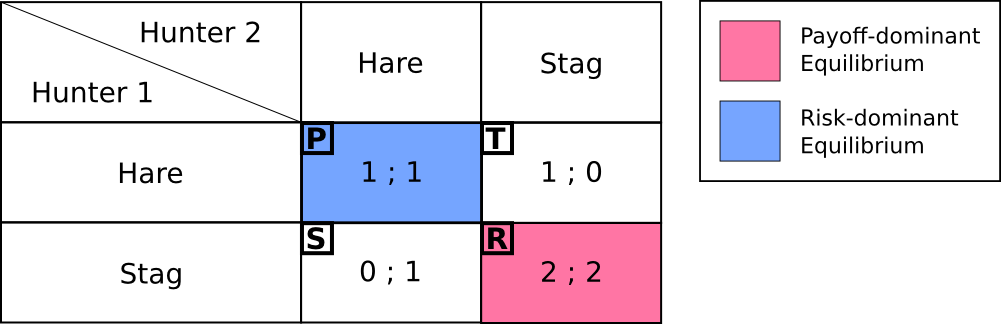
\includegraphics[scale = 0.50]{fig/Intro/StagHunt.png}
          \caption{\textbf{Payoff matrix of the stag hunt.} 
          In the stag hunt~\parencite{Skyrms2004}, we consider that during hunting, two hunters can either hunt a hare or a stag. Hunting a hare can be done in a solitary or cooperative fashion, which ensures that any individual who hunts gets a reward. In comparison, hunting stag can only be achieved in a cooperative fashion but rewards more than a hare. In consequence, an individual who would hunt a stag alone would not get any benefit from hunting. Payoffs are indicated in pair so that we have (Payoff for hunter 1; Payoff for hunter 2). The exact payoffs do not matter as long as the different situations are in that order: R (reward for cooperation) > T (temptation for defection) = P (punishment for defection) > S (sucker's payoff). The payoff-dominant equilibrium is the equilibrium where the hunters maximize their maximum payoff whereas the risk-dominant equilibrium is the one where they maximize their minimum payoff.} 
          \label{fig:MatrixStagHunt}
        \end{center}
    \end{figure}

    The particularity of this game is that there are two evolutionary stable Nash equilibria~\parencite{Nash1950, MaynardSmith1973}. This means that when both individuals hunt hare or when both individuals hunt stag, either strategy is stable against the invasion of mutants. More precisely, this implies that in comparison to the prisoner's dilemma, when the cooperative equilibrium is evolved (hunting stag), its stability is not threatened by the invasion of "defectors" (hare hunters). Thus, in coordination games, cooperation is stable when evolved but risky when rare~\parencite{Forber2015}. The stag hunt is thus appropriate given the context of this manuscript. Namely, we can use this framework to study the emergence of cooperative actions when faced with a bootstrapping problem rather than their stability.

    But as previously said, when we abstract from the mechanics of behaviours as in game theory we may neglect the critical influence of these proximate mechanisms on the evolution of cooperation. When studying the stag hunt we give no explanation on the origin of the coordination mechanisms which allow the individuals to reap the benefits of stag hunting~\parencite{Calcott2007a}. In particular, it is often assumed in game theory that a single mutation is sufficient to switch from one equilibrium to the other. In reality, cooperation cannot be beneficial unless coordination is evolved and coordination is not beneficial on its own. In consequence, the emergence of the cooperative equilibrium entails complex modifications in the behaviours of individuals. Thus the mechanics of these behaviours may impact the evolution of this equilibrium.

    Our aim is thus to model the pratical mechanics of coordination behaviours to study how they influence the ultimate evolution of cooperation. To this end, our approach is that of modeling in \emph{evolutionary robotics}\footnote{The choice of using evolutionary robotics is not without consequences and is not made randomly. In particular, there are critical reasons which justify that we use this technique rather than any other among the numerous modeling frameworks available for evolutionary biology. As this first chapter is a general introduction to this manuscript, we will carefully motivate this choice in Chapter~\ref{chapter:model}. In addition a brief motivation will be provided in the next Section.}~\parencite{Nolfi2000}.


  \subsection{Evolutionary Robotics}

    Evolutionary robotics (ER) is a method based on designing robots by taking a loose inspiration from natural evolution. Namely, ER takes the concepts of \emph{selection} and \emph{variation} in order to explore the complex space of candidate solutions for the design of a whole robotic systems. The idea of using evolutionary processes in order to solve engineering problems is not new. The whole field of evolutionary computing was created on this idea and offered success in optimization problems where more classical methods fail~\parencite{Holland1975, Goldberg1989, Eiben2015}. Evolutionary robotics use the same principles to take on the complex task of designing part or all of a complete robot: sensors, morphology and control~\parencite{Nolfi2000, Floreano2008, Doncieux2015a}. Keep in mind that the term "robot" is used loosely here and can refer either to a physical or simulated robot. This does not impact the general method of evolutionary robotics.

    % TODO: Dire que l'EC c'est cool pour les black box trucs ?

    \begin{figure}[hbt]
        \begin{center}
          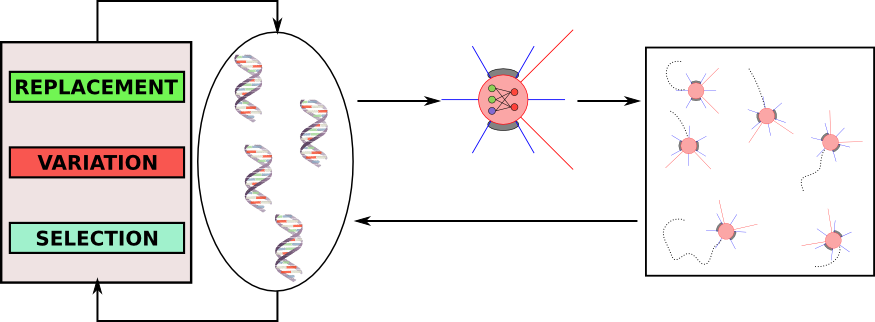
\includegraphics[scale = 0.50]{fig/Intro/EvolutionaryRobotics.png}
          \caption{\textbf{General workflow of an evolutionary robotics algorithm.}
          The main goal of ER is to evolve a population of genotypes. To that end, each genotype must be evaluated to obtain a fitness score. A genotype is thus translated into a phenotype (here an artifical neural network) and then embedded into a robot to act as its controller. The robot is situated in its environment and his behaviour is evaluated in accordance to the specifities of the task. Once every genotype has been asigned a fitness score, they undergo an evolutionary algorithm. This process select the genotypes deemed fit to create offspring, on which variation is then applied. Finally this new population of genotypes replace the previous population and the process can go on for a new generation.} 
          \label{fig:EvolutionaryRobotics}
        \end{center}
    \end{figure}

    Evolutionary robotics is constituted of an evolutionary algorithm whose goal is to evolve a population of artificial genotypes according to a fitness function (see Figure~\ref{fig:EvolutionaryRobotics}). While the actual format of the genotypes is of no particular interest here, it is but rarely similar to a real genotype in both complexity and features. One classical choice in ER is to use a randomly generated collection of real values for each genotype but some other popular choices are to use booleans (e.g. genetica algorithms) or trees (e.g. genetic programming)~\parencite{Eiben2015}. This genotype is then translated into a phenotype which constitutes the robot's morphology and/or control. Again, the transition from genotype to phenotype as well as the actual phenotype itself can both vary greatly from one model to another. On that matter, one must choose what best fits his/her needs. The important point is that in ER this is the phenotype which is evaluated. To that end, the robot is situated in its environment and let to interact with the environment and sometimes other robots. 

    % This principle of designing a robot in the context of its environment and the interactions it has with it is known as \emph{embodied intelligence}~\parencite{Pfeifer2007}.
    
    In the more classical models, a fitness function is used to compute the fitness score based on the behaviour of the robot in its environment. For example, in one of the first experiments where an evolutionary process was used to automatically design the control of a robot~\parencite{Floreano1994}, the goal was for a robot to navigate a looping maze. As such, the fitness function that had to be maximized was designed as follows:

    \[
      F = V(1-\sqrt{\delta v})(1-i)
    \]

    where (1) $V$ is the average rotation speed of the wheels, (2) $\delta v$ is the absolute difference between the speeds of the wheels and (3) $i$ the normalized maximum activation value between every sensors (where these sensors were infrared sensors capable of detecting obstacles). Thus, the goal of the robot was to (1) maximize its translational speed, (2) minimize its rotational speed and (3) minimize the activation of its sensors. So, to put it more simply, its goal was to move (1) as fast as possible (2) as straight as possible and (3) by avoiding obstacles at the same time. A large part of designing an evolutionary robotics algorithm may be spent carefully crafting the fitness function to evolve the behaviour of the robot according to that desired (which is a challenge on its own). However a recent shift occurred in the field toward algorithms that do not rely on a complex and handcrafted fitness function. Rather there is a strong interest in methods that go beyond the focus on objective functions to concentrate on the search for novelty~\parencite{Lehman2008, Lehman2011} or diversity~\parencite{Mouret2012a} in the behaviours evolved. Lastly, it is interesting to note that in most instances of evolutionary algorithm, fitness is thus used to guide the evolutionary process. This is obviously contrary to the biological definition of fitness which is an \emph{a posteriori} observation of the capacity to produce offspring. 

    % While we will but briefly touch upon this subject in our manuscript, it is interesting to know that a few works in evolutionary robotics have been interested in this more "biologically realistic" approach to evolution. In the field of \emph{environment-driven} evolutionary robotics, multiple robots are evolved in open environments where the robotic agents need to encounter other agents so that they can exchange genetic material. Therefore, the selection pressures come from the environment and evolution is driven by the capacity to survive and produce offspring rather than by a fitness score~\parencite{Ray1991, Bianco2004, Bredeche2010}.

    After genotypes have been evaluated, there needs to be the insertion of new individuals in the population. This can be done in a generational fashion, where most or all of the population is replaced at each generation or in a steady state manner, where only a few selected individuals are removed from the population and replaced by new individuals. In order to decide which genotypes will be able to produce offspring and create these new individuals, a selection scheme based on the fitness score is applied. Some of the most popular methods for the selection of individuals are \((\mu + \lambda)\)-ES, \emph{fitness proportionate} and \emph{tournament-based} selection. The first two methods will be thoroughly described in the next Section. As an example, we want to quickly describe the process of tournament-based selection. Under this scheme, an offspring results from a tournament between several (from two to population size minus one) randomly chosen genotypes in the population. These genotypes are then ranked by fitness score. Next the "winning" genotype is selected based on a given paramater $T$. A random value $p$ is then generated. If \(p < T\) then the best genotype is selected. Otherwise we select one of the other genotypes with the same method. This parameter is used to tackle the tradeoff between exploration and exploitation. It is often absent from tournament-based selection as the size of the tournament can also address this dilemma.

    Variation is then finally applied on the offspring to create the population of the next generation. Variation can consist of mutations and/or crossover. A mutation is the process of randomly choosing one or several genes in the genotype, for example according to a uniform distribution, whose value is then randomly changed (in the way that depends from the format of the genotype). In comparison, crossover is used to mix the genotypes of two different offspring. In the most classical way to do crossover, one point crossover, a random point is selected in the genotype and genetic material is swapped between two individuals around this point. Numerous operators of variation exist and depends on the problem at hand.

    % Finally, the population of the new generation is created and the evolution process can go on as long as needs be.

    % When every genotype in the population has been evaluated, a selection scheme is applied based on the fitness score to decide which genotypes will be able to produce offspring for the next generation. For example, a popular method to select the genotypes is to use \emph{tournament-based} selection. Under this scheme, an offspring results from a tournament between several (from one to the population size) randomly chosen genotypes in the population. These genotypes are then ranked by fitness score and each of the genotypes have a certain probability to be selected. Thus, given a certain probability $p$, the best ranked individual is chosen under probability $p$, then the second best ranked individual under probability $p(p-1)$ and so on. This process is repeated until the desired number of offspring have been generated. Variation is then finally applied on these offspring to create the population of the next generation. Variation can consist of mutations and/or crossover. A mutation is the process of randomly chosing one or several genes in the genotype, for example according to an uniform distribution, whose value is then randomly changed (in the way that depends from the format of the genotype). In comparison, the crossover is used to mix the genotypes of two different offspring. In the most classical way to do crossover, one point crossover, a random point is selected in the genotype and genetic material is swapped between two individuals around this point. Finally, the population of the new generation is created and the evolution process can go on as long as needs be.

    In this thesis, we are interested in the modeling of proximate mechanisms in the evolution of mutually beneficial actions. As such, evolutionary robotics is a suitable approach in this context. In particular, ER focus on the modeling of individual-level behaviours resulting from the evolved genotypes situated in a defined environment. This allows to take into account interactions with both the environment and other individuals under complex ecological features. As such, ER has been used to address specific biological hypothesis with a strong emphasis on the mechanistic constraints at play in these evolutionary phenomena~\parencite{Floreano2010, Mitri2013}. Several recent works demonstrated the usefulness of ER in this context by investigating for example the evolution of cooperation~\parencite{Waibel2011, Waibel2009}, the evolution of communication~\parencite{Mitri2011, Wischmann2012} or division of labour~\parencite{Ferrante2015}. Each one of these works will be carefully reviewed in Chapter~\ref{chapter:model}, where we will also provide a more detailted justification of our modeling choice. In consequence, ER is a fitting choice in modeling the proximation mechanisms of coordination and studying their impact on the evolution of cooperation: the mechanics of behaviours are not considered to be a black box anymore.

    Around the common basis of the evolution of coordination, we also want to address an additional problem which is the design of cooperative robots. This is another manner in which evolutionary robotics can contribute to scientific research~\parencite{Trianni2014b, Doncieux2015a}. In particular, ER is a useful approach when designing multi-robots systems. The design of multi-robots systems is complex because it implies to take into account the interactions between multiple individuals in order to produce the emergence of collective functionnalities. The automatic design of robot control with classical learning methods in particular is difficult because of the sheer complexity produced by the size of the problem. In comparison, ER can be used as a black-box optimization technique which does not need to make approximations about the problem at hand. In consequence, several works have focused on designing multi-robots systems with ER, be it for the design of robot swarms~\parencite{Baldassarre2007}, the evolution of specialization~\parencite{Ferrante2015} or the design of flying communicative robots~\parencite{Hauert2014}. In this manuscript we thus focus on the automatic design of multi-robots systems in evolutionary robotics. In particular, we study the influence of team composition (i.e. homogeneity or heterogeneity of individuals) on the evolution of cooperative robots~\parencite{Waibel2009}. We will introduce this problem more thoroughly in Chapter~\ref{chapter:design}.


  \subsection{Experimental Setting}

    We are interested in the dual objective of both modeling the evolution of cooperation and designing multi-robots systems with an evolutionary robotics approach. Both these aspects are independent and may be considered separate problems. However these two aspects share the common problem of the nature of coordination behaviours in the evolution of cooperation and as such we use a similar setting for each of them. In particular, our inspiration is the framework of the stag hunt which we model in evolutionary robotics. As previously explained, this gives us the possibility to model the mechanistic constraints at play in the evolution of mutually beneficial cooperation. However it also acts as an appropriate inspiration for our study of designing multi-robots systems. In particular, we want to investigate the nature of coordination behaviours between heterogeneous robots (in terms of robot control) and the influence of such team composition on the evolution of cooperation when selfish behaviours are possible. In consequence, while both our problems are separate we chose to use a similar (or at least strongly similar) experimental setting for each of these approaches. In this Section, we present this setting. Please note that, as they may change depending on the exact experiments presented in this manuscript, some of the parameter values are not specified in this Section (see Table~\ref{table:tableParameters}). All the parameters that we present have been chosen after conducting preliminary studies.

    \begin{table*}[ht]
      \centerfloat
        \begin{tabular}{|l|l|c|}
          \hline
          \multicolumn{2}{|l|}{\textbf{Parameter}} & \textbf{Value} \\
          \hline
          \textbf{Evolutionary Algorithm} & & \\
          % \hline
          % & Selection method & Fitness-proportionate or \((\mu + \lambda)\)-ES\\
          \hline
          & Per locus mutation probability & \(5 \times 10^{-3}\) \\
          \hline
          & Mutation operator & Gaussian \(\mathcal{N}(0, 0.01)\) \\
          \hline
          & Number of partners & 5 \\
          \hline
          & Number of simulations per pair & 5 \\
          \hline

          \textbf{Artificial Neural Network} & & \\
          \hline
          & Input neurons & 49 \\
          \hline
          & Hidden neurons & 8 \\
          \hline
          & Output neurons & 2 \\
          \hline

          \textbf{Simulation} & & \\
          \hline
          & Simulation duration (in time steps) & 20000 \\
          \hline
          & Capture duration (in time steps) & 800 \\
          \hline
        \end{tabular}
        \caption{\textbf{Experimental parameters.}}
      \label{table:tableParameters}
    \end{table*}

    \subsubsection{Robot model} We want to study the evolution of simulated robotic agents (see Figure~\ref{fig:RobotModel}). These agents are capable of movement thanks to two independant wheels and are equiped with a collection of sensors. Those sensors are of two types: $12$ \emph{proximity sensors} and a $90$ degrees front \emph{camera}. On the one hand, the proximity sensors are equally distributed all around the robot's body and return the proximity of any obstacle nearby (i.e. in a radius which equals twice of the body's diameter) to the agent. On the other hand, the camera cannot recognize the obstacles but can feed the agent with the type of any objects it sees in the environment (including other agents). More precisely, this camera is composed of $12$ rays with an infinite range equally divided in the camera's angle. When one of these rays intersects with an object, it returns the type of this object and its proximity. The robot is thus constituted of simple sensory capabilities. The choice of having the robot model constituted of two different sensory feedback is not innocent. By dividing the sensory capabilities between the proximity sensors and the camera, we are essentially facilitating the process of evolving two basic skills necessary for the robot: obstacles avoidance and agents recognition. This design is not to be considered as a realistic approach to evolution but rather as a way to ease the acquisition of these skills that are of no particular interest here. Furthermore, while the obstacles avoidance mechanism is not expected to improve much during evolution, the appearance of cooperative behaviours in comparison should lead to variation on the manner with which to recognize agents.

    \begin{figure}[hbt]
        \begin{center}
          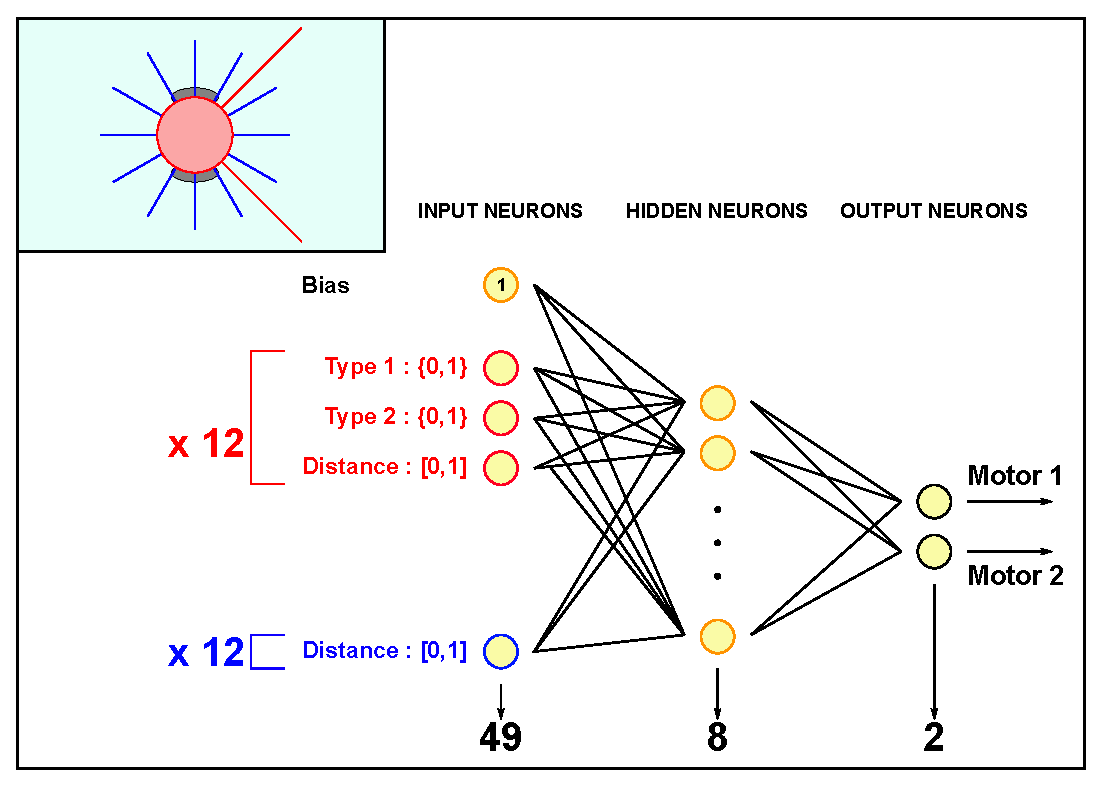
\includegraphics[scale = 0.60]{fig/Intro/RobotModel.eps}
          \caption{\textbf{Robot model of our experimental setting.}
          This figure represents the sensory and neural architecture of simulated robotic agent used in our experimental study. On the robot diagram, proximity sensors are represented by the blue lines whereas the front camera is shown as a red cone. The neural network is a multilayer perceptron with one hidden layer and whose inputs are constituted of all the sensory information of the individual. The outputs of the neural networks are the speeds of both of the robot's wheels.} 
          \label{fig:RobotModel}
        \end{center}
    \end{figure}

    \subsubsection{Controller} The controller of the agent is an artificial neuron network (ANN). While a lot of different types of controllers are used in evolutionary robotics, ANN are widely employed for their versatility~\parencite{Doncieux2015a}. The principle behind a very basic neural network is that it is constituted of a layer of input neurons and a layer of output neurons which are connected (sometimes fully) to each other. Each of the connection has a value, which is called a connection weight. The value of each output neuron is computed as the sum of the input neurons connected to it weighted by the connection weight. A transfer function can then be applied to this output to compute the final value. ANN are really diverse in how they are implemented and can include recurrence or have their topology evolve~\parencite{Stanley2002}.

    In our case, we use a fully connected multilayer perceptron with one hidden layer. This neural network is composed of two outputs which are used to compute the speed of each of the robot's wheels. The inputs of the network are constituted of all the sensory information of the robot in addition to a bias neuron whose value is always $1$. This amounts to a total number of $49$ input neurons: $1$ for each proximity sensors, $3$ for each camera ray and $1$ for bias. The information of each camera is encoded by $3$ neurons as we use $2$ bits to encode the type of each object (hare, stag or the other agent) and $1$ last neuron for the proximity of this object. The hidden layer is constituted of $8$ neurons. Finally, the transfer function used in each neuron is a sigmoid and the topology of the ANN is never changed throughout evolution.

    \subsubsection{Environment} We place two evolved robots in an arena with four solid walls. This arena is filled with randomly positioned objects of different types, where the type can be recognized by the camera. These objects represent the prey that can be hunted by the individuals in the stag hunt game. The objects cannot move while the robots can move freely. We conducted preliminary experiments with moving objects but it was shown that this did not significantly impact the behaviours of the individuals. Additionally, the presence of multiple stationary objetcs already implies that the individuals need to evolve coordination. In consequence, the addition of objects motion is not critical for the conduct of our study.

    In order to catch an object, an individual needs to move to this object and then stay next to it for a specified amount of time steps ($800$ time steps out of $20000$). After this duration, the object is removed from its position and replaced at another random position in the environment; we thus ensure a constant ratio of each type of object. For cooperation to occur, both robots need to be close to the object at the end of this duration. This thus implies that robots need to display actual coordination behaviours in order to be able to cooperate. This also means that an individual can reap the benefits of cooperation simply by being there at the very last step of the capture period.

    An object is always removed if an individual is next to it after this period of time, regardless of wether it requires cooperation. All that varies are the rewards given to the individuals. Please note that, even in the case of cooperation, we do not study the way rewards are distributed between individuals: they are both equally rewarded.

    \subsubsection{Evolutionary algorithm} The genotype of each individual is constituted of all of the connection weights of the neural network. Each gene is initially randomized in the interval where it takes its values, i.e. in \([0,1]\). To evolve these genotypes we use a very classical evolutionary algorithm. At each generation of the algorithm we evaluate each individual of the population in the arena presented before. Its partner is randomly selected in the population. To ensure that each individual encounters a fair sample of the population, each individual is separatly paired with $5$ different partners. From a biological perspective, this means that encounters between individuals are rare w.r.t. the life of a given individual. Then a pair of individuals interact in the arena during $20000$ time steps. In order to decrease the effect due to the stochasticity in the objects' random positioning, each pair plays $5$ different simulations. Thus, each individual plays a total number of $25$ simulations. Fitness is obtained by computing the average reward of the individual in these simulations.

    The individuals are then selected to produce offspring. Throughout our experiments, we mainly studied two different selection methods: \emph{fitness proportionate} and \emph{elitist}. The former is the more classical one when modeling evolutionary biology because it corresponds to a Wright-Fisher model~\parencite{Wright1931} with constant population size. Under this model, we randomly sample through the population to select a parent to create each offspring that will constitute the population of the next generation. Each individual in the population has a higher probability to be selected if its fitness is higher. Each individual can also be selected several times. The latter selection scheme is implemented as a \((\mu + \lambda)\) evolution strategy. With this selection method, we always keep the $\mu$ best individuals of each generation for the next generation. Then we add $\lambda$ offspring to the population of the next generation, where the parents of these offspring are taken from the $\mu$ best individuals ranked by fitness score. In the case of biological modeling, fitness-proportionate is thus a more realistic choice. However, we observed that the elistist selection strategy would reach similar results as fitness proportionate but with smaller population sizes. Thus it allowed to decrease the computational time of our experiments.

    % Justifier mieux Elitist p/r à Fitprop ?

    Whatever the selection strategy, we always create the offspring in the same way. Each offspring is a mutated clone of its parent. Then mutation is applied independently on each gene according to a mutation rate of \(5 \times 10^{-3}\). If a gene mutates, mutation is sampled according to a gaussian distribution \(\mathcal{N}(0, 0.01)\). Lastly, we use no recombination (i.e. crossover) in any of our experiments. Because this thesis is focused on cooperation between unrelated individuals (in model as in design), it raises no particular issue to limit variation to mutations.


\section{Evolving Coordination in Evolutionary Robotics}

  While this introduction was mainly focused on the biological aspect of cooperation and the problem its origin poses for evolutionary biology, we want to study several facets under this general problem. As we previously talked about, we believe that our approach in evolutionary robotics entails that the contributions of this thesis can serve different purposes around the common subject of the evolution of coordination. Historically, evolutionary robotics has been used at its inception for the automatic design of robotic systems. However, there has been a real debate on how the works in this field could really contribute to scientific research as well as to whom it may be of interest~\parencite{Trianni2014b, Doncieux2015a}. It is now admitted that reseach in evolutionary robotics should be clearly directed toward either of two goals: modeling biological questions or designing robots~\parencite{Trianni2014b}. In this thesis, our goal is to present different contributions which separately aim for each of these goals. In this last Section, we briefly present the structure of the manustript.
  
  \subsection{Modeling the Evolution of Coordination}

    In the first section of this manuscript, we use evolutionary robotics in order to model the evolution of cooperation. Because we tend to generally ignore or minimize the pratical mechanics of behaviour, the role of coordination in the evolution of collective mutualistic actions is often underestimated. Yet, the proximate mechanisms of coordination may influence the convergence to a cooperative solution. We thus study how the nature of coordination behaviours and the mechanisms that underlie their evolution may impact the ultimate evolution of cooperation. The particular issue we address here could be summarized as follows: \emph{what are the proximate mechanisms which hinder or facilite the ultimate evolution of mutualistic cooperation ?}

    %TODO: un moyen de faire mieux ressortir la problématique ?

    To that end, we will spend some time in the introduction of this section to motivate our choice regarding evolutionary robotics, something we deliberately skipped in this general introduction. One reason why the proximate causes of coordination have often been overlooked is that classical models used for studying evolutionary problems may not be appropriate for this particular goal. We believe that among the distinct assumptions made by these models, some are critical if we plan to fully understand the evolution of coordination. However, it is important to make clear that we do not pretend our approach to be a more realistic depiction of nature. Rather we claim that, while we still study a theoretical abstraction of cooperative actions, the assumptions behind our model allow us to study particular mechanisms we believe of importance for this issue.


  \subsection{Designing Cooperative Robots}

    In the second section of the manuscript, we want to study the evolution of cooperation in a team of heterogeneous robots. In consequence, we focus on the automatic design of multirobots systems. As we will explain more in details in Chapter~\ref{chapter:design}, multirobots systems have now been investigated for a long time for their advantages over single robots. In particular, they may allow to design more efficient and cheaper robotic systems as well as benefit from the redundancy of multiple robots to design more robust systems. Moreoever, it can simply sometimes be necessary to coordinate several robots at the same time to achieve a particular task. The practical applications of such systems are numerous, in particular in environments where humans cannot go and where using a single and generally more complex robot would simply not be reliable enough. As such, multirobot systems could be used for collective manipulation, building or exploration of hazardous environments. For example, cooperative robots could investigate and perform repairs inside nuclear plants after particularly catastrophic incidents.

    However, designing this sort of systems is challenging. It is one thing to engineer a factory robot which is programmed to perform a very specific and repetitive task in a controled environment. It is another to design a robot capable of acting in an uncertain environment and able to adapt to the unexpected. And even more complicated when multiple robots must both possess the qualities expected from a single robot and also coordinate in an efficient manner. Multiple techniques for automatic design have been proposed, in particular for the control of robots. However, when it comes to adaptability to changing environment and uncertainty, the "easiest" way is to design a robot that is capable to learn from previous experiences. Among the learning methods used in this context, ER is a promising one when robots are expected to perform in an open and changing environment. Therefore we explore how ER can be used for the auomatic design of collective robots. 

    % This choice will be dutifully justified in this section of the manuscript. 

    We are interested in the nature of the coordination behaviours that could be evolved between heterogeneous individuals. Heterogeneous teams of robots allow for more diverse behaviours to emerge inside a group of individuals. However, while there has always been a clear interest on adding heterogeneity in multirobots systems~\parencite{Parker1994, Parker2008}, most research on the evolution of cooperative robots have been focused on homogeneous groups of individuals (which is equivalent to the mechanism of kin selection under maximum genetic relatedness)~\parencite{Waibel2009}. This is indeed one of the safiest way to ensure that robots will indeed evolve a cooperative behaviour, as there is no selfish interest to act in a solitary fashion. However, we believe that the influence of heterogeneity on the quality of the coordination behaviours is as much of importance as the capacity to evolve a cooperation solution. In particular, when coordination is needed, heterogeneity may lead to more efficient cooperative behaviours. However, conflict can arise from the selfish interests of the individuals. Thus, the issue we focus on in this second Part of the manuscript is: \emph{how can we evolve efficient coordination behaviours in a group of heterogeneous cooperative robots ?}


  \subsection{Organization of the Manuscript}

    This thesis is comprised of two Parts that each address one of the two problems we described here. Each Part is composed of an introduction Chapter and two results Chapters. Each of the results Chapters begins with a short introduction and quick summary of the results presented in the Chapter. After both part, a final concluding Chapter is present.
    Chapter $2$ presents a brief overview of the modeling techniques used in evolutionary robotics and for the evolution of cooperation in particular. The goal is to provide the reader with a justification about our choice to use evolutionary robotics to model the evolution of cooperation.
    Chapter $3$ is presented as an article published in an international journal. It focuses on the comparison between a classical game theoretical analysis of the stag hunt and the results we obtained with our evolutionary robotics model.
    Chapter $4$ is shown as the draft for a future journal article. This Chapter addresses the issue of the optimization of collective actions by way of individual selection and the impact of the nature of coordination strategies in that context.
    Chapter $5$ briefly presents the field of multirobot systems and the review the different methods used in designing the control of distributed robots. The design problem of evolving cooperation between heterogeneous robots is then described.
    Chapter $6$ reads as an article published in an international conference. It focuses on a comparison between clonal and aclonal approach in a cooperative foraging task with regards to evolvability and efficiency.
    Chapter $7$ is presented as another article published in an international conference. It deals with the evolution of specialization at the level of population, i.e. the evolution of genotypic polymorphism.
    Finally, Chapter $8$ summarizes our contributions and addresses their limits as well as the perspectives it opens for future research.
